% http://www.springer.de/comp/lncs/authors.htm
% max 20 pages
%\documentclass{llncs}
%\usepackage[letterpaper,tmargin=1.5in,bmargin=1.5in,lmargin=1.5in,rmargin=1.5in]{geometry}

%\usepackage[T1]{fontenc}



%\usepackage{hyperref}
%\usepackage{fixltx2e}





%\usepackage[english]{babel}
%\usepackage{vmargin} \setpapersize{USletter} \setmarginsrb{4cm}{4.5cm}{4cm}{2.8cm}{5mm}{5mm}{5mm}{10mm}

%% \setcounter{tocdepth}{4}
%% \setcounter{secnumdepth}{4}
%% \def\ssp{\def\baselinestretch{.98}\large\normalsize}

%% \ssp

%\clubpenalty=10000
%\widowpenalty=10000

\hyphenation{pu-bli-sh-ed}


\newcommand{\acunetix}{Acunetix}
\newcommand{\appscan}{AppScan}
\newcommand{\burp}{Burp}
\newcommand{\grendelscan}{Grendel-Scan}
\newcommand{\hailstorm}{Hailstorm}
\newcommand{\milescan}{Milescan}
\newcommand{\nstalker}{N-Stalker}
\newcommand{\ntospider}{NTOSpider}
\newcommand{\paros}{Paros}
\newcommand{\webinspect}{Webinspect}
\newcommand{\waf}{w3af}

\newcommand{\initial}{INITIAL}
\newcommand{\config}{CONFIG}
\newcommand{\manual}{MANUAL}


%% \begin{document}

%% \frontmatter

%% \title{Why Johnny Can't Pentest:\\
%% An Analysis of Black-box Web Vulnerability Scanners}

%% \author{Adam Doup\'e\ \and Marco Cova \and Giovanni Vigna}
%% \institute{University of California, Santa Barbara\\
%%   \email{\{adoupe,marco,vigna\}@cs.ucsb.edu}}

%% \date{}

%% \maketitle

%% \begin{abstract}

%% Black-box web vulnerability scanners are a class of tools that can be
%% used to identify security issues in web applications. These tools are
%% often marketed as ``point-and-click pentesting'' tools that
%% automatically evaluate the security of web applications with little or
%% no human support. These tools access a web application in the same way
%% users do, and, therefore, have the advantage of being independent of the
%% particular technology used to implement the web application. However,
%% these tools need to be able to access and test the application's various
%% components, which are often hidden behind forms, JavaScript-generated
%% links, and Flash applications.

%% This paper presents an evaluation of eleven black-box web
%% vulnerability scanners, both commercial and open-source.  The evaluation
%% composes different types of vulnerabilities with different challenges to
%% the crawling capabilities of the tools. These tests are integrated in a
%% realistic web application.  The results of the evaluation show that
%% crawling is a task that is as critical and challenging to the overall
%% ability to detect vulnerabilities as the vulnerability detection
%% techniques themselves, and that many classes of vulnerabilities are
%% completely overlooked by these tools, and thus research is required to 
%% improve the automated detection of these flaws.
%% \end{abstract}

\section{Why Johnny Can't Pentest}

Web application vulnerabilities, such as cross-site scripting and SQL
injection, are one of the most pressing security problems on the
Internet today. In fact, web application vulnerabilities are widespread, accounting
for the majority of the vulnerabilities reported in the Common
Vulnerabilities and Exposures database~\cite{cve}; they are 
frequent targets of automated attacks~\cite{small08predator}; and, if
exploited successfully, they enable serious attacks, such as data
breaches~\cite{datalossdb} and drive-by-download
attacks~\cite{provos08iframes}. 
In this scenario, security testing of web applications is clearly
essential.  

% web applications and their security problems

%Today, web applications  are the preferred means to
%offer services online and are routinely used by millions of users to
%perform both mundane and sensitive tasks, such as interacting with banking
%systems, accessing governmental services, and buying goods online. 
%
%Unfortunately, web applications are not free from design and
%implementation defects, which can be abused by malicious
%users to perform attacks that compromise the security of the
%application itself or the confidentially and integrity of the data it handles. In fact, in the past years,
%most of the vulnerabilities reported in the Common Vulnerability and
%Exposure database affected web applications~\cite{cve}. This situation is further
%worsened by the constantly changing technologies, the heterogeneity of
%implementation languages and browsers, the \emph{ad hoc} nature of most
%web applications, and the lack of proper security
%training of web developers. As a consequence, there exist a large
%number of vulnerable web applications that are publicly deployed.

% software engineering practices and regulations demand testing of web
% applications

A common approach to the security testing of web applications consists
of using {\em black-box web vulnerability scanners}.
%A common approach to the security testing of web
%applications is {\em black-box} testing, in which a live version of the
%application is exercised with a variety of inputs and its responses are
%analyzed to detect unexpected behaviors and identify vulnerabilities. 
%% common approach: black-box testing via web application scanners
%In practice, black-box security testing of  web applications is
%performed by using {\em web application vulnerability scanners}. 
These are tools that
%, starting from a few pages that act as seeds,  
crawl a web
application to enumerate all the reachable pages and the associated input vectors
(e.g., HTML form fields and HTTP GET parameters), generate specially-crafted input
values that are submitted to the application, and observe the
application's behavior (e.g., its HTTP responses) to determine if a
vulnerability has been triggered.

Web application scanners have gained popularity, due to
their independence from the specific web application's technology, ease of
use, and high level of automation. (In fact, web application scanners
are often marketed as ``point-and-click'' pentesting tools.) In the past
few years, they have also become a requirement in several standards,
most notably, in the Payment Card Industry Data Security
Standard~\cite{pci}.

%  In fact, they do not require access to the source code of
%the web application under test, and, therefore, they are independent of
%the specific technology and programming language used to implement it.
%In addition, they can operate in automatic or semi-automatic fashion,
%and, thus, they can be managed by a system administrator or tester with
%limited security training. (In fact, web application scanners are often
%marketed as ``point-and-click'' pentesting tools.)
%Finally, web application scanners are 
%recommended to achieve compliance with security
%standards, most notably the Payment Card Industry Data Security
%Standard~\cite{pci}. 

Nevertheless, web application scanners have limitations. 
Primarily, as most testing tools, they provide no guarantee of
soundness.
%While this may appear just a theoretical concern, 
Indeed, in the last few years, several reports have shown that
state-of-the-art web application scanners fail to detect a significant
number of vulnerabilities in test applications~\cite{suto07,suto10webscanners,wiegenstein06,peine06,anantasec09}.
These reports are valuable, as they warn against the naive use of web
application scanners (and the false sense of security that derives from
it), enable more informed buying decisions, and  prompt to rethink
security compliance standards. 

However, knowing that web application scanners miss vulnerabilities (or
that, conversely, they may raise false alerts) is only part of the
question. Understanding {\em why} these tools have poor detection
performance is critical to gain insights into how current tools work and
to identify open problems that require further research.  
%
More concretely, we seek to determine the root causes of the
errors that web application scanners make, by considering all the phases
of their testing cycle, from crawling, to input selection, to response
analysis.
%
For example, some of the questions that we want to
answer are: Do web application scanners correctly handle JavaScript
code? Can they detect vulnerabilities that are ``deep'' in the
application (e.g., that are reachable only after correctly submitting
complex forms)? Can they precisely keep track of the state of the
application?

%Crawling, attack, analysis.
%The main drawback of web application scanners
%is that they can miss vulnerabilities for three reasons: (i) they
%might not be able to reach the page from where a vulnerability can be triggered,
%(ii) they do not use the ``right'' input value necessary to trigger
%the vulnerability, or (iii)
%they are not able to determine if the attack is successful. These are particularly serious
%issues when testing modern web applications, 
%which are often complex software artifacts that
%integrate different client-side technologies (e.g., HTML, JavaScript,
%and Flash), require sophisticated user interaction (e.g., to correctly
%fill in forms with several input fields), and implement multi-step
%workflows (e.g., when filling carts and performing payments during a purchase). 
%Crawling these applications can be a challenging task \emph{per se}.
%Furthermore, scanners must exercise an application with inputs that
%satisfy the validity checks enforced by the application but still
%cause the vulnerability to manifest (for example, with either a crash or an
%error message).

%Unfortunately, up to now, little has been done to assess the
%state-of-the-art of web application scanners. More precisely,  
%a number of questions remain open with regard to their ability to
%effectively and efficiently scan modern, feature-rich web applications. 
%For example, do web application scanners correctly handle JavaScript
%code? Can they detect vulnerabilities that are ``deep'' in the
%application (e.g., that are reachable only after correctly
%submitting forms)? Can they precisely keep track of the state of the
%application?

To do this, we built a realistic web application, called WackoPicko, and used it
to evaluate eleven web application scanners on their ability to crawl
complex web applications and to identify the associated vulnerabilities. 
%
More precisely, the WackoPicko application uses features that are
commonly found in modern web applications and that make their crawling
difficult, such as complex HTML forms, extensive JavaScript and Flash code,
and dynamically-created pages.
%
Furthermore, we introduced in the application's source code a number of
vulnerabilities that are representative of the bugs commonly found in
real-world applications.
%
The eleven web application scanners that we tested include both commercial
and open-source tools. We evaluated each of them under three different
configuration settings, corresponding to increasing levels of manual
intervention.
%
We then analyzed the results produced by the tools in order to
understand how the tools work, how effective they are, and what makes
them fail. The ultimate goal of this effort is to identify which tasks
are the most challenging for black-box vulnerability scanners and may
require novel approaches to be tackled successfully. 

The main contributions of this paper are the following:
\begin{compactitem}
\item We performed the most extensive and thorough evaluation of black-box 
web application vulnerability scanners so far.
\item We identify a number of challenges that scanners
need to overcome to successfully test modern web applications both in terms
of crawling and attack analysis capabilities.
\item We describe the design of a testing web site for web application
scanners that composes crawling challenges with vulnerability instances.
This site has been made available to the public and can be used by other
researchers in the field.
\item We analyze in  detail \emph{why} the web application vulnerability
  scanners succeed or fail and we identify areas that need further research.
\end{compactitem}


\section{Background}

Before discussing the design of our tests, it is useful to briefly discuss the
vulnerabilities that web application scanners try to identify and to present
an abstract model of a typical scanner.

\subsection{Web Application Vulnerabilities}

Web applications contain a mix of traditional flaws (e.g.,
ineffective authentication and authorization mechanisms) and web-specific
vulnerabilities (e.g., using user-provided inputs in SQL queries 
without proper sanitization). Here, we will briefly describe some of the
most common vulnerabilities in web applications (for further details,
the interested reader can refer to the OWASP Top 10 List,
which tracks the most critical vulnerabilities in web
applications~\cite{owasptopten}):
%The most common cause of vulnerabilities in web applications is the 
%lack of proper validation of parameters that are passed by the client to
%the application~\cite{owasptopten}. This weakness can be leveraged to perform
%several different attacks, depending on the context in which the vulnerability is
%present.
\begin{compactitem}
\item {\bf Cross-Site Scripting (XSS): }
% definition
XSS vulnerabilities allow an attacker to execute malicious JavaScript
code as if the application sent that code to the user. 
% consequences
This is the first most serious vulnerability of the OWASP Top 10 List,
and WackoPicko includes five different XSS vulnerabilities, both
reflected and stored.

\item {\bf SQL Injection: }
% definition
SQL injection vulnerabilities allow one to manipulate, create or execute
arbitrary SQL queries.
This is the second most serious vulnerability on the OWASP Top 10 List, and
the WackoPicko web application contains both a reflected and a stored SQL injection
vulnerability.

\item {\bf Code Injection: }
% description
Code injection vulnerabilities allow an attacker to execute arbitrary
commands or execute arbitrary code.
This is the third most serious vulnerability on the OWASP Top 10 List, and
WackoPicko includes both a command line injection and a file inclusion
vulnerability (which might result in the execution of code).

\item {\bf Broken Access Controls: }
% definition
A web application with broken access controls fails to properly define
or enforce access to some of its resources.
% attack
This is the tenth most serious vulnerability on the OWASP Top 10
List, and
WackoPicko has an instance of this kind of vulnerability.

\end{compactitem}

\subsection{Web Application Scanners}

In abstract, web application scanners can be seen as consisting of three
main modules: a {\em crawler} module, an {\em attacker} module, and an {\em analysis} module.
The crawling component is seeded with a set of URLs,
retrieves the corresponding pages, and follows links and redirects to
identify all the reachable pages in the application.
In addition, the crawler identifies all the input points to the application,
such as the parameters of GET requests, the input fields of HTML forms,
and the controls that allow one to upload files.

The attacker module analyzes the URLs discovered by the crawler and the
corresponding input points. Then, for each input and for each
vulnerability type for which the web application vulnerability scanner
tests, the attacker module generates values
that are likely to trigger a vulnerability. For example,
the attacker module would attempt to inject JavaScript code when testing for XSS
vulnerabilities, or strings that have a special meaning in the SQL language, such as ticks and SQL operators, when testing for SQL
injection vulnerabilities.
Input values are usually generated using heuristics or using predefined
values, such as those contained in one of the many available XSS and
SQL injection
cheat-sheets~\cite{rsnake:sql_cheat_sheet,rsnake:xss_cheat_sheet}.

The analysis module analyzes the pages returned by the web application in
response to the attacks launched by the attacker module to detect possible
vulnerabilities and to provide feedback to the other modules.  For example, if
the page returned in response to input testing for SQL injection contains a
database error message, the analysis module may infer the existence of a SQL
injection vulnerability.



\section{The WackoPicko Web Site}

A preliminary step for assessing web application scanners consists of
choosing a web application to be tested. We have three requirements for
such an application: it must have clearly defined vulnerabilities (to
assess the scanner's detection performance), it must be easily
customizable (to add crawling challenges and experiment with different
types of vulnerabilities), and it must be representative of the web
applications in use today (in terms of functionality and of
technologies used).

We found that existing applications did not satisfy our requirements.
Applications that deliberately contain vulnerabilities, such as
HacmeBank~\cite{hacme_bank} and WebGoat~\cite{owasp-webgoat}, are often
designed to be educational tools rather than realistic testbeds for
scanners. Others, such as SiteGenerator~\cite{owasp_sitegenerator}, are
well-known, and certain scanners may be optimized to perform well on
them.
An alternative then is to use an older version of an open-source
application that has known vulnerabilities. In this case, however, we
would not be able to control and test the crawling capabilities of the
scanners, and there would be no way to establish a false negative
rate. 

% why did we do this instead of our own?
%When choosing a test application, we surveyed well-known
%web applications that contain known vulnerabilities such as HacmeBank,
%WebGoat, and SiteGenerator~\cite{hacme_bank,owasp_sitegenerator,owasp-webgoat}. 
%While representing valuable
%educational tools in their own way, they did not have the
%characteristics necessary to be used as tests in our evaluation. 
%Another alternative is to test the web application vulnerability
%scanners against an older version of an open-source application that
%has known vulnerabilities. However, we wouldn't be able to control and
%test the crawling capabilities of the scanners, and there would be no
%way to establish the false negative rate. We needed a
%web application that had clearly defined vulnerabilities, crawler
%challenges, and was easily customizable. 

Therefore, we decided to
create our own test application, called WackoPicko. It is important to
note that WackoPicko is a realistic, fully functional web application. As
opposed to a simple test application that contains just
vulnerabilities, WackoPicko tests the scanners under realistic conditions.
To test the scanners' support for client-side JavaScript code,
we also used the open source Web Input
Vector Extractor Teaser (WIVET). WIVET is a synthetic benchmark
that measures how well a crawler is able to discover and follow links
in a variety of formats, such as JavaScript, Flash, and form submissions.

\subsection{Design}
WackoPicko is a photo sharing and
photo-purchasing site. A typical
user of WackoPicko is able to upload photos, browse other user's
photos, comment on photos, and purchase the rights to a high-quality
version of a photo.

\noindent {\bf Authentication.}
WackoPicko provides personalized content to registered users.
Despite recent efforts for a unified
login across web sites~\cite{openid}, most web applications require a
user to create an account in order to utilize the 
services offered. Thus, WackoPicko has a user registration
system. Once a user has created an account, he/she can log in to
access WackoPicko's restricted features. 

\noindent {\bf Upload Pictures.} 
When a photo is uploaded to
WackoPicko by a registered user, other users can comment on it, as well as purchase
the right to a high-quality version.

\noindent {\bf Comment On Pictures.} 
Once a picture is uploaded into WackoPicko, all registered users can
comment on the photo by filling out a form.
Once created, the comment is displayed, along with the picture,
with all the other comments associated with the picture.

\noindent {\bf Purchase Pictures.} 
A registered user on WackoPicko can purchase the high-quality version
of a picture. The purchase follows a multi-step process in which a shopping cart
is filled with the items to be purchased,  similar to the process used
in e-commerce
sites. After pictures are added to the cart, the
total price of the cart is reviewed, discount coupons may be applied, and the
order is placed. Once the pictures are purchased, the user 
is provided with links to the high-quality version of the pictures.

\noindent {\bf Search.} 
To enable users to easily search for various pictures,
WackoPicko provides a search toolbar at the top of every
page. The search functionality utilizes the tag field that was filled out when
the picture was uploaded. After a query is issued, the user is
presented with a list of all the pictures that have tags that
match the query. 

\noindent {\bf Guestbook.} 
A guestbook page provides a way to receive feedback from all visitors
to the WackoPicko web site. The form used to submit feedback contains a ``name'' field and
a ``comment'' field. 

\noindent {\bf Admin Area.} 
WackoPicko has a special area for administrators only, which has a
different login mechanism than regular users. 
Administrators can perform special actions, such as
deleting user accounts, or changing the tags of a picture.

\subsection{Vulnerabilities}

The WackoPicko web site contains sixteen vulnerabilities that are
representative of vulnerabilities found in the wild, as reported by the 
OWASP Top 10 Project~\cite{owasptopten}.
%In WackoPicko the vulnerabilities can be
%split into two broad classes: those vulnerabilities that require a valid login to be
%exploited, and those that do not. 
In the following we provide a brief description of each vulnerability.

\subsubsection{Publicly Accessible Vulnerabilities}
A number of vulnerabilities
in WackoPicko can be exploited without first logging into the web
site.\\

\noindent {\bf Reflected XSS:}
There is a XSS vulnerability on the search page, which is accessible without
having to log into the application. In fact, the query parameter is not
sanitized before being echoed to the user. The presence of the vulnerability
can be tested by setting the query parameter to
{\tt<script>alert('xss')</script>}. When this string is reflected to the user,
it will cause the browser to display an alert message. (Of course, an
attacker would leverage the vulnerability to perform some malicious
activity rather than alerting the victim.)

\noindent {\bf Stored XSS:}
There is a stored XSS vulnerability in the
guestbook page. The {\tt comment} field is not properly escaped, and therefore, an
attacker can exploit this vulnerability by creating a comment containing
JavaScript code.
Whenever a user visits the
guestbook page, the attack will be triggered and the (possibly
malicious) JavaScript code executed.

\noindent {\bf Session ID:} 
The session information associated with administrative accounts is handled
differently than the information associated with the sessions of normal users.
The functionality associated with normal users uses PHP's session handling
capabilities, which is assumed to be free of any session-related
vulnerabilities (e.g., session fixation, easily-guessable session IDs).
However the admin section uses a custom session cookie to keep track of sessions.
The value used in the cookie is a non-random value that is incremented when a
new session is created. Therefore, an attacker can easily guess the session id
and access the application with administrative rights.

\noindent {\bf Weak password:} 
The administrative account page has an easily-guessable
username and password combination: admin/admin.

\noindent {\bf Reflected SQL Injection:} 
WackoPicko contains a reflected SQL injection in the {\tt user\-name}
field of the login form. By introducing a tick into
the {\tt username} field it is possible to perform arbitrary queries in the 
database and obtain, for example, the usernames and passwords of
all the users in the system.

\noindent {\bf Command Line Injection:} 
WackoPicko provides a simple service that
checks to see if a user's password can be found in the dictionary. The 
{\tt password} parameter of the form used to request the check is used
without sanitization in the shell command: {\tt grep \verb|^|<password>\$ 
/etc/dictionaries-common/words}. This can be exploited by providing as
the password value a
dollar sign (to close grep's regular expression), followed by a semicolon (to
terminate the grep command), 
followed by extra commands.

\noindent {\bf File Inclusion:} 
The admin interface is accessed through a main page, called {\em index.php}.
The index page acts as a portal; any value that is passed as its
{\tt page} parameter will be concatenated with
the string ``.php'', and then
the resulting PHP script will be run. For instance, the URL for the admin login page is
{\tt /admin\-/index.php?\-page=login}. On the server side, \emph{index.php} will
execute \emph{login.php} which displays the form. This design is inherently flawed, because it
introduces a file inclusion vulnerability. An attacker can
exploit this vulnerability and execute remote PHP code by supplying, for
example,  {\tt
  http://hacker/\-blah.php\%00} as the {\tt page} parameter to \emph{index.php}.
The {\tt \%00} at the end of the string causes PHP to ignore the ``.php'' that
is appended to the page parameter. Thus \emph{index.php} will download and
execute the code at \url{http://hacker/blah.php}.

%Note: do I have to use the %00?? It looks to me that if I pass just
%http://hacker.com/blah, the url http://hacker.com/blah.php will be requested
% This is important because we say that the lack of the %00 is what caused the 
% scanner to miss the attack
%ANote: No, don't have to use a %00 and http://hacker.com/blah will
%work but how would the scanner know this? The %00 is the only way a
%scanner would be able to reliably test for something getting appended
%after the input parameter.
\noindent {\bf Unauthorized File Exposure:} 
In addition to executing remote code, the file inclusion vulnerability can
also be exploited to expose local files. Passing {\tt/etc/passwd\%00} as the
``page'' GET parameter to \emph{index.php} of the admin section will cause the
contents of the {\tt/etc/passwd} file to be disclosed.

\noindent {\bf Reflected XSS Behind JavaScript:} 
On WackoPicko's home page there is a form that checks if a file is in the proper
format for WackoPicko to process. This form has two parameters, a file
parameter and a name parameter. Upon a successful upload, the name is echoed
back to the user unsanitized, and therefore, this represents a
reflected vulnerability.
However, the form is dynamically generated using JavaScript, and the target of
the form is dynamically created by concatenating strings. This prevents
a crawler from using simple pattern matching to discover the URL
used by the form.

\noindent {\bf Parameter Manipulation:} 
The WackoPicko home page provides a
link to a sample profile page. The link uses the ``userid'' GET parameter to view
the sample user (who has id of 1). An attacker can manipulate this variable
to view any profile page without having a valid user account.

\subsubsection{Vulnerabilities Requiring Authentication}
A second class of vulnerabilities in WackoPicko can be exploited only
after logging into the web site.\\


\noindent {\bf Stored SQL Injection:} 
When users create an account, they are asked to supply their first name.
This supplied value is then used unsanitized on a page that shows other users who have a
similar first name. An attacker can exploit this vulnerability by
creating a user with the name ``' ; DROP users;\#'' then visiting the
similar users page.


\noindent {\bf Directory Traversal:} 
When uploading a picture, WackoPicko copies the file uploaded by the user to a
subdirectory of the \emph{upload} directory. The name of the subdirectory is the
user-supplied tag of the uploaded picture. A malicious user can manipulate the
tag parameter to perform a directory traversal attack. More precisely, by
pre-pending ``{\tt../../}'' to the tag parameter the attacker can reference files outside
the upload directory and overwrite them.

\noindent {\bf Multi-Step Stored XSS:} 
Similar to the stored XSS attack that exists on the guestbook, comments on
pictures are susceptible to a stored XSS attack. However, this vulnerability
is more difficult to exploit because the user must be logged in and must
confirm the preview of the comment before the attack is actually triggered.

\noindent {\bf Forceful Browsing:} 
One of the central ideas behind WackoPicko is the ability of users to purchase
the rights to high-quality versions of pictures. However, the access to the
links to the high-quality  version of the picture is not checked, and an attacker who acquires the URL of a
high-quality picture can access it without creating an account, thus
bypassing the authentication logic. 

\noindent {\bf Logic Flaw:} 
The coupon
system suffers from a logic flaw, as a coupon can be applied multiple times to
the same order reducing the final price of an order to zero.

\noindent {\bf Reflected XSS Behind Flash:} 
On the user's home page there is a Flash form that asks the user for his/her
favorite color. The resulting
page is vulnerable to a reflected XSS attack, where the ``value'' parameter
 is echoed back to the user without being sanitized.

\subsection{Crawling Challenges}
Crawling is arguably the most important part of a web application
vulnerability scanner; if the scanner's attack engine is poor, it
{\em might} miss a vulnerability, but if its crawling engine is poor and
cannot reach the vulnerability, then it will {\em surely} miss the
vulnerability. Because of the critical nature of crawling, we have included several types of
crawling challenges in WackoPicko, some of which hide vulnerabilities.

\noindent {\bf HTML Parsing.}
Malformed HTML makes it difficult for web application scanners to
crawl web sites. For instance, a crawler must be able to navigate
HTML frames and be able to upload a file. Even though 
these tasks are straightforward for a human user with a regular
browser, they represent a challenge for crawlers. 

\noindent {\bf Multi-Step Process.}
Even though most web sites are built on top of the stateless
HTTP protocol, a variety of techniques are utilized to
introduce state into web applications. In order to properly
analyze a web site, web application vulnerability scanners must
be able to understand the state-based transactions that take
place. In WackoPicko, there are several state-based
interactions. 

\noindent {\bf Infinite Web Site.}
It is often the case that some dynamically-generated content
will create a very large (possibly infinite) crawling space.
For example, WackoPicko has the ability to display a daily calendar. 
Each page of the calendar displays the agenda for a given day and
links to the page for the following day. A crawler that naively followed
the links in the WackoPicko's calendar would end up trying to visit an
infinite sequence of pages, all generated dynamically by the same
component.
%accepts a {\tt date} parameter and generate a page corresponding to the
%provided date.
%timestamp in its {\tt date} parameter and generates a page 
%, in which the ``date'' GET
%parameter is a UNIX timestamp. Each page of the calendar
%includes a link to the ``next day''. This creates
%a large series of pages.

\noindent {\bf Authentication.}
One feature that is common to most web sites is an authentication
mechanism. Because this is so prevalent, scanners must properly handle
authentication, possibly by creating accounts, logging in with valid
credentials, and recognizing actions that log the crawler
out. WackoPicko includes a registration and login system to test the
scanner's crawlers ability to handle the authentication process correctly.

\noindent {\bf Client-side Code.}
Being able to parse and understand 
client-side technologies presents a major challenge for web
application vulnerability scanners. WackoPicko includes
vulnerabilities behind a JavaScript-created form, as well as behind a
Flash application. 

\noindent {\bf Link Extraction.}
We also tested the scanners on WIVET, an open-source 
benchmark for web link extractors~\cite{wivet}.  WIVET contains 54 tests and 
assigns a final score to a crawler based on the percent of tests that 
it passes. The tests require scanners to analyze
simple links, multi-page forms, links in comments
and JavaScript actions on a variety of HTML elements. There are also
AJAX-based tests as well as Flash-based tests. In our tests, we used WIVET 
version number 129.


\section{Experimental Evaluation}

We tested 11 web application scanners  by running them on our WackoPicko
web site. The tested scanners included 8 proprietary tools and 3 open
source programs. Their cost ranges from free to tens of thousands of
dollars. We used evaluation versions of each software, however they
were fully functional.
A summary of the characteristics of the scanners we evaluated is given
in Table~\ref{scanners}.

\begin{table}[t]
  \centering
    \begin{scriptsizetabular}{lp{15em}rrr}
      \hline
      Name & Version Used & License & Type & Price \\
      \hline
      \acunetix & 6.1 Build 20090318 & Commercial & Standalone & \$4,995-\$6,350 \\
      \appscan & 7.8.0.0 iFix001 Build: 570 Security Rules Version 647 & Commercial & Standalone & \$17,550-\$32,500 \\
      \burp & 1.2 & Commercial & Proxy & \pounds125 (\$190.82) \\
      \grendelscan & 1.0 & GPLv3 & Standalone & N/A \\
      \hailstorm & 5.7 Build 3926 & Commercial & Standalone & \$10,000 \\
      \milescan & 1.4 & Commercial & Proxy & \$495-\$1,495 \\
      \nstalker & 2009 - Build 7.0.0.207 & Commercial & Standalone & \$899-\$6,299 \\
      \ntospider & 3.2.067 & Commercial & Standalone & \$10,000 \\
      \paros & 3.2.13 & Clarified Artistic License & Proxy & N/A \\
      \waf & 1.0-rc2 & GPLv2 & Standalone & N/A \\
      \webinspect & 7.7.869.0 & Commercial & Standalone & \$6,000-\$30,000 \\
      \hline
    \end{scriptsizetabular}
    \caption{Characteristics of the scanners evaluated.}
    \locallabel{scanners}
  \end{table}
 
%\vspace{-10ex}

%When looking at black-box web application vulnerability scanners, there are a
%number of characteristics that can be used to compare the
%scanners. One of these characteristics is
%open-source or commercial (proprietary). Open-source scanners 
%allow users to access and modify their source code, and, in addition,
%they are usually free.
%Commercial scanners are usually closed-source and cost from several hundred to tens of thousand of US dollars.
%
%
%Scanners also have different designs.
%There are stand-alone desktop scanners
%whose sole purpose is to scan for different vulnerabilities, and scanners
%that are part of a suite of tools. These suites typically include a proxy
%through which the user can manipulate requests/responses to perform
%manual vulnerability analysis. Once a URL is
%accessed through the proxy, the user can then send that URL to a
%crawler. A set of URLs or an entire site can then be
%sent to a scanner component. In a more streamlined process, a stand-alone desktop scanner is given a starting URL and the tool
%will attempt to find all vulnerabilities on the site. 

We ran the WackoPicko web application on a typical LAMP machine, with
Apache 2.2.9, PHP 5.2.6, and MySQL 5.0.67. We enabled the {\tt
allow\_\-url\_\-fopen} and {\tt allow\_\-url\_\-include}  PHP options and disabled the  {\tt magic\_\-quotes} option.
We ran the scanners on a machine with a Pentium 4 3.6GHz CPU, 1024 MB of
RAM, and Microsoft Windows XP, Service Pack 2.
%The host running the vulnerable web server used in our experiments was
%an Intel Pentium 4 3.6GHz CPU with 512 MB of RAM, 
% running Ubuntu distribution 8.10 with Linux kernel
%version 2.6.27-11-generic. The web server was Apache 2.2.9 with PHP Version 5.2.6-2ubuntu4.1 with {\tt
%  allow\_\-url\_\-fopen} enabled as well as {\tt allow\_\-url\_\-include} and {\tt
%  magic\_\-quotes} disabled. MySQL version 5.0.67 was used as the
%back-end database.
%
%The host that was used to run the scanners was an Intel
%Pentium 4 3.6GHz CPU with 1024 MB of RAM running Microsoft
%Windows XP, Service Pack 2.

\subsection{Setup}
The WackoPicko server used in testing the web vulnerability scanners was run in a virtual
machine, so that before each test run the server could be put in an
identical initial state. This state included ten regular users, nine pictures,
%with five comments on those pictures, 
and five administrator users.

Each scanner was run in three different configuration modes against
WackoPicko, with each configuration requiring more setup on the part of the
user. In all configuration styles, the default values for configuration parameters were used, and when choices
were required, sensible values were chosen. In the \initial{}
configuration mode, the scanner was
directed to the initial page of WackoPicko and told to scan for all
vulnerabilities. In the \config{} setup, the scanner was given a valid
username/password combination or login macro before scanning. 
\manual{} configuration required the most
work on the part of the user; each scanner was put into a ``proxy'' mode
and then the user browsed to each vulnerable page accessible without credentials; then, the user
logged in and visited each vulnerability that required a login.
Additionally a picture was uploaded, the rights to a high-quality version
of a picture were purchased, and a coupon was applied to the order. The
scanner was then asked to scan the WackoPicko web site.

%Before being run against the WIVET benchmark, the variable
%{\tt\$\_SESSION['baseaddr']} in the \emph{genclude.php} file was changed to
%the IP address of the vulnerable server. Once these changes were made to
%the server, the scanner was asked to scan the URL {\tt
%  http://\-wacko\-picko.\-com/\-wivet}  and, if possible, was told to just do a crawl and not inject
%anything. 

%\begin{center}
  \begin{table}[t]
    \centering
    %\begin{minipage}{\textwidth}
    {\scriptsize
      \begin{tabular}{|l|p{11ex}|p{11ex}|p{11ex}|p{11ex}|p{11ex}|p{11ex}|p{11ex}|p{11ex}|}
        \hline
        Name & Reflected XSS  & Stored XSS & \parbox[t]{11ex}{\raggedright Reflected SQL Injection} & \parbox[t]{11ex}{\raggedright Command-line Injection } & \parbox[t]{11ex}{\raggedright File Inclusion } & \parbox[t]{11ex}{\raggedright File Exposure } & \parbox[t]{11ex}{\raggedright XSS via JavaScript } & \parbox[t]{11ex}{\raggedright XSS via Flash }\\
        \hline
        \acunetix{} & \initial{} & \initial{} & \initial{} &  & \initial{} & \initial{} & \initial{} & \\
        \appscan{} & \initial{} & \initial{} & \initial{} &  & \initial{} & \initial{} &  &  \\
        \burp{} & \initial{} & \manual{} & \initial{} & \initial{} &  & \initial{} &  & \manual{} \\
        \grendelscan{} & \manual{} &  & \config{} &  &  &  &  &  \\
        \hailstorm{} & \initial{} & \config{} & \config{} &  &  &  &  & \manual{} \\
        \milescan{} & \initial{} & \manual{} & \config{} &  &  &  &  &  \\
        \nstalker{} & \initial{} & \manual{} & \manual{} &  &  & \initial{} & \initial{} & \manual{} \\
        \ntospider{} & \initial{} & \initial{} & \initial{} &  &  &  &  &  \\
        \paros{} & \initial{} & \initial{} & \config{} &  &  &  &  & \manual{} \\
        \waf{} & \initial{} & \manual{} & \initial{} &  & \initial{} &  &  & \manual{} \\
        \webinspect{} & \initial{} & \initial{} & \initial{} &  & \initial{} &  & \initial{} & \manual{} \\
        \hline
    \end{tabular}}
    \caption{Detection results. For each scanner, the simplest configuration that detected a vulnerability is given. Empty cells indicate no detection in any mode.}
    \locallabel{results}
    %\end{minipage}
    %\begin{minipage}{0.3\textwidth}
    %  {\scriptsize
    %\begin{tabular}{|l|r|r|r|}
    %  \hline
    %  Name & \initial & \config & \manual \\
    %  \hline
    %  \acunetix{} & 1 & 7 & 4 \\
    %  \appscan{} & 11 & 20 & 26 \\
    %  \burp{} & 1 & 2 & 6 \\
    %  \grendelscan{} & 15 & 16 & 16 \\
    %  \hailstorm{} & 3 & 11 & 3 \\
    %  \milescan{} & 0 & 0 & 0 \\
    %  \nstalker{} & 5 & 0 & 0 \\
    %  \ntospider{} & 3 & 1 & 3 \\
    %  \paros{} & 1 & 1 & 1 \\
    %  \waf{} & 1 & 1 & 9 \\
    %  \webinspect{} & 215 & 317 & 297 \\
    %  \hline
    %\end{tabular}}
    %\caption{False positives.}
    %\label{falsepositives}
    %\end{minipage}
  \end{table}
%\end{center}

\subinputfrom{figures/}{results_graph_wrapper}
%\vspace{-10ex}

\subsection{Detection Results}
The results of running the scanners against the WackoPicko site are
shown in Table~\ref{results} and, graphically, in
Figure~\ref{results_graph}.
%
The values in the table correspond to the
simplest  configuration that discovered the vulnerability. An empty cell indicates that
the given scanner did not discover the vulnerability in any
mode. The table only reports the vulnerabilities that were detected by at least one scanner.
%Figure~\ref{results_graph} shows the detection percentage of the
%various scanners when run in each mode. 
%The False Negative percentage
%in Figure~\ref{results_graph} shows the percentage of vulnerabilities
%that the scanner did not find.
Further analysis of why the scanners missed
certain vulnerabilities is contained in Sections~\ref{attack-and-analysis}
and~\ref{crawling}. 

The running time of the scanners is shown in Figure~\ref{running_time_graph}.
These times range from 74 seconds for the fastest tool (\burp{}) to 6
hours (\nstalker{}). The majority of the scanners completed the
scan within a half hour, which is acceptable for an automated tool. 


\subsubsection{False Negatives}

One of the benefits of developing the WackoPicko web application to
test the scanners is the ability for us to measure the false negatives
of the scanners. An ideal scanner would be able to detect all
vulnerabilities. In fact, we had a group composed of students with 
average security skills 
analyze WackoPicko. The students found all vulnerabilities
except for the forceful browsing vulnerability. The automated
scanners did not do as well; there were a number of vulnerabilities
that were not detected by any scanner. These vulnerabilities are
discussed hereinafter.

% SessionID     
\noindent {\bf Session ID: }         
No scanner was able to detect the session ID vulnerability on the
admin login page. The vulnerability was not detected because the scanners were not given a
valid username/password combination for the admin interface. This
is consistent with what would happen when scanning a typical application, as the
administration interface would include powerful functionality that the scanner
should not invoke, like view, create, edit or delete
sensitive user data.
% especially when testing a live site.
The session ID was only set on a
successful login, which is why this vulnerability was not detected by any scanner.

% Note: If I were a reviewer I would say: "I would probably scanned a test
% version of the application and provide the admin login as well"
% I think that the reason that we give for this failure is sort of lame.
% Is it possible to re-run the tests with the login to see if they detect it?
% I don't think that they would be able to detect it anyway...

% Weak Password          
\noindent {\bf Weak Password: }
Even though the scanners were not given a valid username/password combination
for the administrator web site, an administrator account with the
 combination of admin/admin was present on the system.
\ntospider{} was the only scanner that successfully logged in with the
admin/admin combination. However, it did not report it as an error, which
suggests that it was unable to detect that the login was successful, even
though the response that was returned for this request was different from every other login
attempt.

% Parameter Manipulation 
\noindent {\bf Parameter Manipulation: }
The parameter manipulation vulnerability was not discovered by any 
scanner. There were two causes for this: first, only three of the
scanners (\appscan{}, \ntospider{}, and \waf{})
input a different number than the default value ``1'' to the {\tt userid}
parameter. Of the 
three, only \ntospider{} used a value that successfully manipulated the {\tt
  userid} parameter. The other reason  was that in order to
successfully detect a parameter manipulation vulnerability, the scanner needs
to determine which pages require a valid username/password to access and which
ones do not and it is clear that none of the scanners make
this determination.

% SQL Injection Stored   
\noindent {\bf Stored SQL Injection: }
The stored SQL injection was also not discovered by any scanners, due to the
fact that a scanner must create an account to discover the stored SQL
injection. The reasons for this are discussed in more detail in
Section~\ref{ability-create-account}.

% Directory Traversal    
\noindent {\bf Directory Traversal: }
The directory traversal vulnerability was also not discovered by any of the
scanners. This failure is caused by the scanners being unable to
upload a picture. We
discuss this issue in Section~\ref{picture-creation}, when we analyze how each of the
scanners behaved when they had to upload a picture.

% XSS Stored Login
\noindent {\bf Multi-Step Stored XSS: }
The stored XSS vulnerability that required a confirmation step was also missed
by every scanner. In Section~\ref{picture-commenting}, we analyze how many of
the scanners were able to successfully create a comment on a picture.

% Forceful Browsing      
\noindent {\bf Forceful Browsing: }
No scanner found the forceful browsing vulnerability, which is not 
surprising since it is an application-specific
vulnerability. These vulnerabilities are difficult to identify
without access to the source code of the application~\cite{balzarotti07mimosa}.

% Logic Flaw - Coupon    
\noindent {\bf Logic Flaw: }
Another vulnerability that none of the scanners uncovered was the
logic flaw that existed in the coupon management functionality. 
%It is
%fairly evident that no scanner was able to discover this
%vulnerability, because 
Also in this case, some domain knowledge about the application is needed to
find the vulnerability.



\begin{table}[tb]
  \centering
  \begin{tabular}{|l|r|r|r|}
    \hline
    Name & \initial & \config & \manual \\
    \hline
    \acunetix{} & 1 & 7 & 4 \\
    \appscan{} & 11 & 20 & 26 \\
    \burp{} & 1 & 2 & 6 \\
    \grendelscan{} & 15 & 16 & 16 \\
    \hailstorm{} & 3 & 11 & 3 \\
    \milescan{} & 0 & 0 & 0 \\
    \nstalker{} & 5 & 0 & 0 \\
    \ntospider{} & 3 & 1 & 3 \\
    \paros{} & 1 & 1 & 1 \\
    \waf{} & 1 & 1 & 9 \\
    \webinspect{} & 215 & 317 & 297 \\
    \hline
  \end{tabular}
  \caption{False positives.}
  \locallabel{falsepositives}
\end{table}

%\vspace{-10ex}

\subsubsection{False Positives}

The total number of false positives for each of the scanning
configurations are show in Table~\ref{falsepositives}.
 %and graphically represented in Figure~\ref{false_positives_graph}.  
The number 
of false positives that each scanner generates is an important metric, because
the greater the number of false positives, the less useful the tool is to the
end user, who has to figure out which of the vulnerabilities reported are actual
flaws and which are spurious results of the analysis. 

The majority of the false positives across all scanners were due to a supposed
``Server Path Disclosure.'' This is an information leakage vulnerability where
the server leaks the paths of local files, which might give an attacker 
hints about the structure of the file system.

An analysis of the results identified two main reasons why these
false positives were generated. The first is that while testing the
application for file traversal or file injection vulnerabilities, some of the scanners passed
parameters with values of file names, which, on some pages (e.g., the guestbook page),
caused the file name to be included in that page's contents. When the
scanner then tested the page for a Server Path Disclosure, it found
the injected values in the page content, and generated a Server Path Disclosure
vulnerability report. 
The other reason for the generation of false positives is that WackoPicko uses
absolute paths in the {\tt href} attribute of anchors (e.g.,
{\tt/users/home.php}), which the scanner mistook for the disclosure of paths in
the local system. 
\webinspect{} generated false positives because of both the above reasons, which explains the
large amount of false positives produced by the tool. 

Some scanners reported
genuine false positives: \hailstorm{} reported a false XSS vulnerability and two
false PHP code injection vulnerabilities, \ntospider{} reported three false XSS
vulnerabilities and \waf{} reported a false PHP {\tt eval()} input injection
vulnerability.

\subsubsection{Measuring and Comparing Detection Capabilities}
% first talk about the dominates figure and what that means.

Comparing the scanners using a single benchmark like WackoPicko does
not represent an exhaustive evaluation. However, we believe that the results
provide insights about the current state of black-box web application
vulnerability scanners.

One possible way of comparing the results of the scanners is arranging them in a
lattice. This lattice is ordered on the basis of \emph{strict
  dominance}. Scanner A \emph{strictly dominates} Scanner B if and only if for
every vulnerability discovered by Scanner B, Scanner A discovered that
vulnerability with the same configuration level or simpler, and Scanner A either
discovered a vulnerability that Scanner B did not discover or Scanner A discovered a
vulnerability that Scanner B discovered, but with a simpler configuration.
\emph{Strictly dominates} has the property that any assignment of scores to
vulnerabilities must preserve the \emph{strictly dominates} relationship.

%\begin{center}
  \begin{figure}[t]
    \begin{minipage}{.5\textwidth}
%      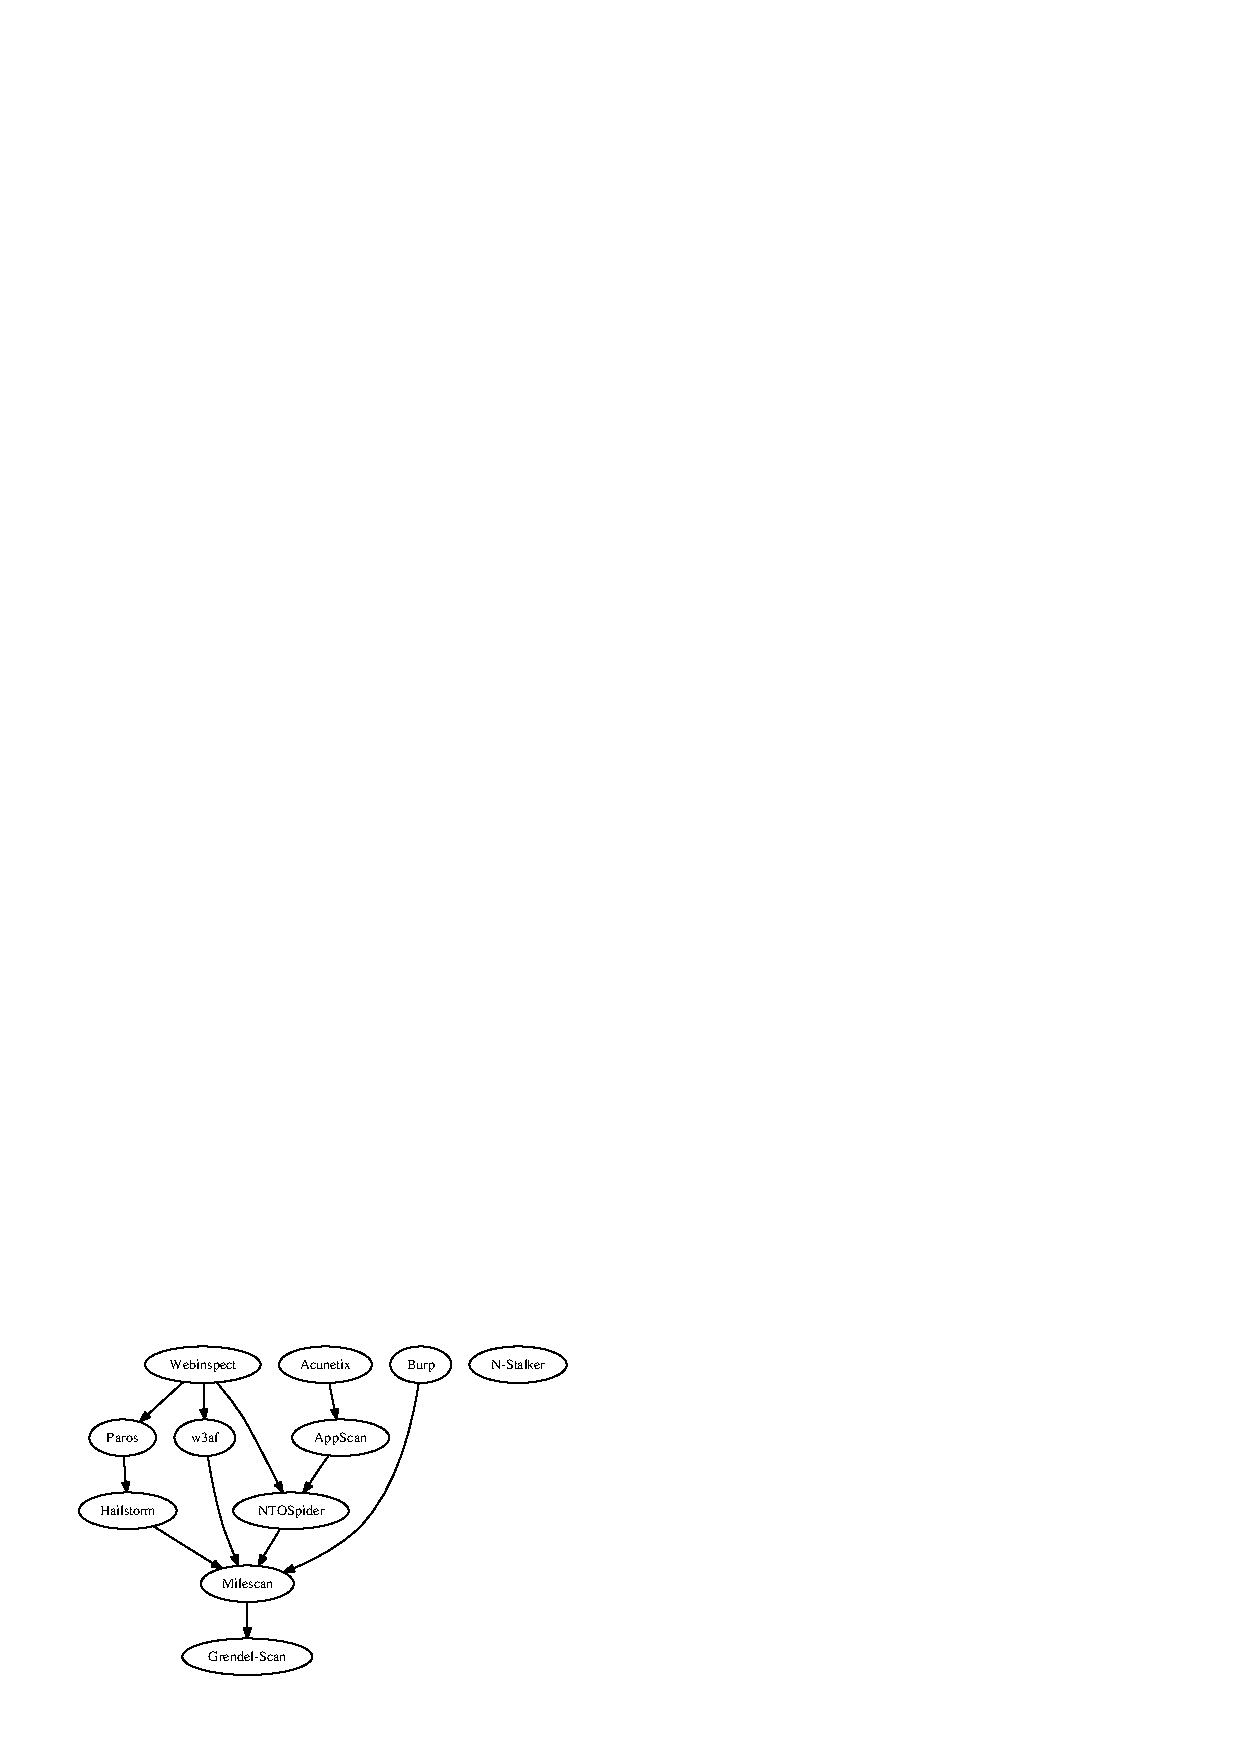
\includegraphics[scale=.80]{all_results_rank}
      \caption{Dominates graph.}
      \label{domgraph}
    \end{minipage}
    \begin{minipage}{.5\textwidth}
%      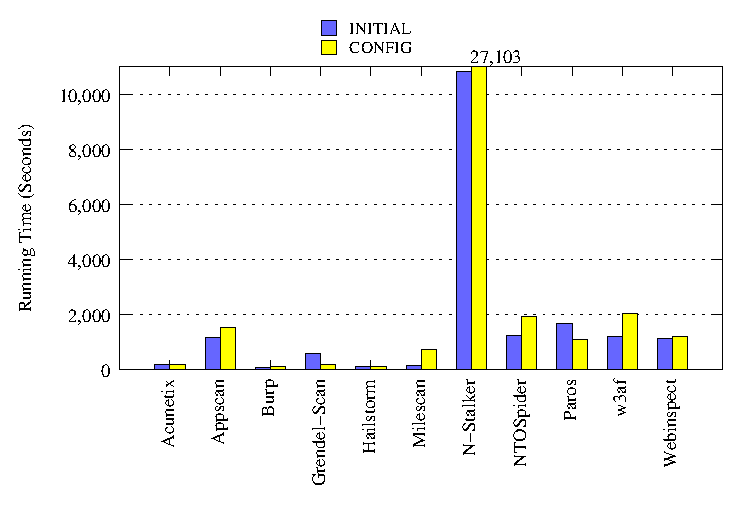
\includegraphics[scale=.5]{running_time_graph}
      \caption{Scanner Running Times}
      \label{running_time_graph}
    \end{minipage}
  \end{figure}
%\end{center}

%\vspace{-10ex}

Figure \ref{domgraph} shows the \emph{strictly dominates} graph for the
scanners, where a directed edge from Scanner A to Scanner B means
that Scanner A \emph{strictly dominates} Scanner B. Because \emph{strictly
  dominates} is transitive, if one scanner \emph{strictly dominates} another
it also \emph{strictly dominates} all the scanners that the dominated
scanner dominates, therefore, all redundant edges are not
included. Figure \ref{domgraph} is organized so that the scanners in
the top level are 
those that are not \emph{strictly dominated} by any scanners. Those in the
second level are strictly dominated by only one scanner and so on, until the
last level, which contains those scanners that strictly dominate no other scanner.

Some interesting observations arise from Figure \ref{domgraph}. \nstalker{}
does not strictly dominate any scanner and no scanner strictly dominates it.
This is due to the unique combination of vulnerabilities that \nstalker{}
discovered and missed.
%
\burp{} is also interesting due to the fact that it only dominates two
scanners but no scanner dominates \burp{} because it was the only
scanner to discover the command-line injection vulnerability. 

  \begin{table}[t]
      {\scriptsize
        \begin{tabular}{|p{25ex}|l|p{12ex}|p{12ex}|p{12ex}|}
          \hline
          Name                             &  Detection  &  \initial{} Reachability  &  \config{} Reachability  &  \manual{} Reachability  \\
          \hline
          XSS Reflected                    &       1  &             0  &            0  &            0  \\
          XSS Stored                       &       2  &             0  &            0  &            0  \\
          SessionID                        &       4  &             0  &            0  &            0  \\
          SQL Injection Reflected          &       1  &             0  &            0  &            0  \\
          Commandline Injection            &       4  &             0  &            0  &            0  \\
          File Inclusion                   &       3  &             0  &            0  &            0  \\
          File Exposure                    &       3  &             0  &            0  &            0  \\
          \parbox[t]{25ex}{\raggedright XSS Reflected behind JavaScript}  &       1  &             3  &            3  &            0  \\
          Parameter Manipulation           &       8  &             0  &            0  &            0  \\
          Weak password                    &       3  &             0  &            0  &            0  \\
          SQL Injection Stored Login       &       7  &             7  &            3  &            3  \\
          Directory Traversal Login        &       8  &             8  &            6  &            4  \\
          XSS Stored Login                 &       2  &             8  &            7  &            6  \\
          Forceful Browsing Login          &       8  &             7  &            6  &            3  \\
          Logic Flaws - Coupon             &       9  &             9  &            8  &            6  \\
          XSS Reflected behind flash       &       1  &             9  &            7  &            1  \\
          \hline
      \end{tabular}}
      \caption{Vulnerability scores.}
      \locallabel{vulnscores}
  \end{table}


%\subsubsection{Scoring}
%  talk about the vulnerability difficulty table
While Figure~\ref{domgraph} is interesting, it does not give a way to compare
two scanners where one does not strictly dominate the other. In order to
compare the scanners, we assigned scores to each vulnerability present in
WackoPicko. The scores are displayed in Table~\ref{vulnscores}. The ``Detection''
score column in Table~\ref{vulnscores} is how many points a
scanner is awarded based on how difficult it is for an automated tool to detect the existence of the
vulnerability. In addition to the ``Detection'' score, each
vulnerability is assigned a ``Reachability'' score, which indicates how difficult
the vulnerability is to reach (i.e., it reflects the difficulty of crawling to the page that contains the vulnerability). 
There are three ``Reachability'' scores for
each vulnerability, corresponding to how difficult it is for a scanner to
reach the vulnerability when run in \initial{}, \config{}, or \manual{} mode.
Of course, these vulnerability scores are subjective and depend on the
specific characteristics of our WackoPicko application. However, their
values try to estimate the crawling and detection difficulty of each
vulnerability in this context.

\begin{table}[tb]
      \centering
      \begin{tabular}{|l|r|}
        \hline
        Name           &  Score  \\
        \hline
        \acunetix      &     14  \\
        \webinspect    &     13  \\
        \burp          &     13  \\
        \nstalker      &     13  \\
        \appscan       &     10  \\
        \waf           &      9  \\
        \paros         &      6  \\
        \hailstorm     &      6  \\
        \ntospider     &      4  \\
        \milescan      &      4  \\
        \grendelscan   &      3  \\
        \hline
      \end{tabular}
      \caption{Final ranking.}
      \locallabel{finalranking}
\end{table}



% then talk about the final scores
The final score for each scanner is calculated by adding up the ``Detection''
score for each vulnerability the scanner detected and the ``Reachability'' score
for the configuration (\initial{}, \config{} and \manual{}) used when
running the scanner. In the case of a tie, the scanners were ranked
by how many vulnerabilities were discovered in \initial{} mode, which
was enough to break all ties. Table~\ref{finalranking} shows the
final ranking of the scanners.

%\vspace{-10ex}

\subsection{Attack and Analysis Capabilities}
\label{attack-and-analysis}
% initial talk of detection methods, what to do when you have multiple
% parameters
Analyzing how each scanner attempted to detect vulnerabilities gives
us insight into how these programs work and  illuminates areas for
further research. First, the scanner would crawl the site
looking for injection points, typically in the form of GET or POST parameters.
Once the scanner identifies all the inputs on a page, it then attempts to inject
values for each parameter and observes the response. When a page
has more than one input, each parameter is injected in turn, and generally no
two parameters are injected in the same request. However, scanners differ in
what they supply as values of the non-injected parameters: some have a
default value like {\tt 1234} or {\tt Peter Wiener}, while others leave the
fields blank. This has an impact on the results of the scanner, for
example the WackoPicko guestbook requires that both the {\tt name} and {\tt
  comment} fields are present before making a comment, and thus the strategy
employed by each scanner can affect the effectiveness of the
vulnerability scanning process.

% XSS Attack
When detecting XSS attacks, most scanners employed similar techniques, some with
a more sophisticated attempt to evade possible filters than others. One particularly
effective strategy employed was to first input random data with various
combinations of dangerous characters, such as {\tt /\ ,",',<, and >}, and then, if
one of these combinations was found unchanged in the response, to attempt the
injection of the full range
of XSS attacks. This
technique speeds up the analysis 
significantly, because the full XSS attack is not attempted
against every input vector. Differently, some of the scanners took an
exhaustive 
approach, attempting the full gamut of attacks on every combination of inputs.


When attempting a XSS attack, the thorough scanners would inject the
typical {\tt <script> alert('xss') </script>} as well as a whole range
of XSS attack strings, such as JavaScript in a tag with the {\tt
  onmouseover} attribute, in an {\tt img}, {\tt div} or {\tt meta}
tag, or {\tt iframe}. Other scanners attempted to evade
filters by using a different JavaScript function other than {\tt alert}, or by
using a different casing of {\tt script}, such as {\tt ScRiPt}.

% Unsanitized Input
Unlike with XSS, scanners could not perform an easy test
to exclude a parameter from thorough testing for other Unsanitized Input
vulnerabilities because the results
of a successful exploit might not be readily evident in the response. This is
true for the command-line injection on the WackoPicko
site, because the output of the injectable command was not used in the
response. 
\burp{}, the only scanner that was able to successfully detect the command line
injection vulnerability, did so by injecting {\tt `ping -c 100 localhost`} and noticing that
the response time for the page was much slower than when nothing was injected.

This pattern of measuring the difference in response times was also
seen in detecting SQL injections. In addition to injecting something with a
SQL control character, such as tick or quote and seeing if an error is
generated, the scanners also used a time-delay SQL injection,
inputting {\tt
  waitfor delay '0:0:20'} and seeing if the execution was
delayed. This is a variation of the technique of using time-delay SQL
injection to extract database information from a blind SQL vulnerability.

%% talk about file-exposure
When testing for File Exposure, the scanners were typically the same; however
one aspect caused them to miss the WackoPicko vulnerability. Each scanner that
was looking for this vulnerability input the name of a file that they knew
existed on the system, such as {\tt /etc/passwd} on UNIX-like systems or {\tt
  \verb|C:\boot.ini|} for Windows. The scanners then looked for known strings
in the response. The difficulty in exploiting the WackoPicko file exposure was
including the null-terminating character ({\tt \%00}) at the end of
the string, which caused PHP to ignore 
anything added by the application after the {\tt /etc/passwd} part. The results show that only 4
scanners successfully discovered this vulnerability.

% Remote Code Execution
The remote code execution vulnerability in WackoPicko is similar to the file exposure
vulnerability. However, instead of injecting known files, the scanners injected
known web site addresses. This was typically from a domain the scanner's developers
owned, and thus when successfully exploited, the injected page appeared
instead of the regular page. The same difficulty in a successful exploitation
existed in the File Exposure vulnerability, so a scanner had to add {\tt \%00}
after the injected web site. Only 3 scanners were able to successfully
identify this vulnerability.

%\begin{center}
  \begin{table*}[t]
    {\scriptsize
%      \begin{tabular}{|l|p{14ex}|p{14ex}|p{14ex}|p{14ex}|p{14ex}|p{14ex}|p{14ex}|p{14ex}|p{8ex}|p{10ex}|p{8ex}|}
      \begin{tabular}{|l|p{8ex}p{8ex}p{10ex}|p{4ex}p{4ex}p{5ex}|p{4ex}p{4ex}p{5ex}|p{4ex}p{4ex}p{5ex}|p{4ex}p{4ex}p{5ex}|p{4ex}p{4ex}p{5ex}|}
        \hline
        Name & \multicolumn{3}{|c|}{Reflected XSS} & \multicolumn{3}{|c|}{Stored XSS} & \multicolumn{3}{|p{14ex}|}{Reflected SQL Injection} & \multicolumn{3}{|p{15ex}|}{Command-line Injection} & \multicolumn{3}{|p{14ex}|}{File Inclusion / File Exposure / Weak password} & \multicolumn{3}{|p{14ex}|}{XSS Reflected - JavaScript} \\
            & \initial{} & \config{} & \manual{} & & & & & & & & & & & & & & &  \\
          \acunetix{} & 496&638&498   & 613&779&724   & 544&709&546   & 495&637&497   & 198&244&200   & 670&860&671   \\
          \appscan{} & 581&575&817   & 381&352&492   & 274&933&628   & 189&191&288   & 267&258&430   & 0&0&442   \\
          \burp{} & 256&256&207   & 192&192&262   & 68&222&221   & 68&68&200   & 125&316&320   & 0&0&178   \\
          \grendelscan{} & 0&0&44   & 1&1&3   & 14&34&44   & 1&1&3   & 2&2&5   & 0&0&2   \\
          \hailstorm{} & 232&229&233   & 10&205&209   & 45&224&231   & 180&160&162   & 8&204&216   & 153&147&148   \\
          \milescan{} & 104&0&208   & 50&0&170   & 75&272&1237   & 0&0&131   & 80&0&246   & 0&0&163   \\
          \nstalker{} & 1738&1162&2689   & 2484&2100&3475   & 2764&1022&2110   & 2005&1894&1987   & 1437&2063&1824   & 1409&1292&1335   \\
          \ntospider{} & 856&679&692   & 252&370&370   & 184&5&5   & 105&9&9   & 243&614&614   & 11&13&13   \\
          \paros{} & 68&68&58   & 126&126&110   & 151&299&97   & 28&28&72   & 146&146&185   & 0&0&56   \\
          \waf{} & 157&157&563   & 259&257&464   & 1377&1411&2634   & 140&142&253   & 263&262&470   & 0&0&34   \\
          \webinspect{} & 108&108&105   & 631&631&630   & 297&403&346   & 164&164&164   & 239&237&234   & 909&909&0   \\
          \hline
          Name & \multicolumn{3}{|c|}{Parameter Manipulation} & \multicolumn{3}{|p{14ex}|}{Directory Traversal} & \multicolumn{3}{|p{14ex}|}{Logic Flaw} & \multicolumn{3}{|p{14ex}|}{Forceful Browsing} & \multicolumn{3}{|p{14ex}|}{XSS Reflected behind flash} & & & \\
          \acunetix{} & 2&0&2   & 35&1149&37   & 0&0&5   & 0&0&206   & 1&34&458 & & & \\
          \appscan{} & 221&210&222   & 80&70&941   & 0&0&329   & 0&0&71   & 0&0&243 & & & \\
          \burp{} & 192&194&124   & 68&68&394   & 0&0&314   & 0&0&151   & 0&0&125 & & & \\
          \grendelscan{} & 3&3&6   & 1&1&3   & 0&0&6   & 0&0&1   & 0&0&3 & & & \\
          \hailstorm{} & 3&143&146   & 336&329&344   & 131&132&5   & 102&102&105   & 0&0&143 & & & \\
          \milescan{} & 105&0&103   & 8&0&163   & 0&0&1   & 0&0&60   & 0&0&68   & & & \\
          \nstalker{} & 1291&1270&1302   & 22&2079&4704   & 0&0&3   & 0&0&2   & 0&0&1315 & & & \\
          \ntospider{} & 107&115&115   & 11&572&572   & 0&11&11   & 0&0&0   & 0&11&11 & & & \\
          \paros{} & 72&72&72   & 14&14&0   & 0&0&114   & 0&0&70   & 0&0&60 & & & \\
          \waf{} & 128&128&124   & 31&30&783   & 0&0&235   & 0&0&270   & 0&0&119 & & & \\
          \webinspect{} & 102&102&102   & 29&29&690   & 0&8&3   & 0&118&82   & 0&0&97 & & & \\
          \hline
        \end{tabular}}
        \caption{Number of accesses to vulnerable web pages in \initial{}, \config{}, and \manual{} modes.}
        \label{access}
  \end{table*}
%\end{center}




%\vspace{-10ex}

\subsection{Crawling Capabilities}
\label{crawling}

The number of URLs requested and accessed varies considerably among scanners,
depending on the capability and strategies implemented in the crawler and
attack components. Table~\ref{access} shows the number of times each scanner
made a {\tt POST} or {\tt GET} request to a vulnerable URL when the scanners
were run in \initial{}, \config{}, and \manual{} mode.
%, and gives an overview of
%how much of WackoPicko each scanner was able to explore. 
For instance, from
Table~\ref{access} we can see that \hailstorm{} was able to access many of the
vulnerable pages that required a valid username/password when run in \initial{} mode. It
can also be seen that \nstalker{} takes a shotgun-like approach to scanning;
it has over 1,000 accesses for each vulnerable URL, while in contrast
\grendelscan{} never had over 50 accesses to a vulnerable URL.  

In the following, we discuss the main challenges that the crawler components of the
web application scanners under test faced.


\subsubsection{HTML}
The results for the stored XSS attack reveal some interesting characteristics of
the analysis performed by the various scanners. For instance, \burp{}, \grendelscan{}, \hailstorm{},
\milescan{}, \nstalker{}, and \waf{} were unable to discover the stored XSS
vulnerability in \initial{} configuration mode. \burp{} and \nstalker{} failed
because of defective HTML parsing. Neither of the scanners correctly
interpreted the {\tt <textarea>} tag as an input to the HTML form. This
was evident because both scanners only sent the {\tt name} parameter when
attempting to leave a comment on the guestbook. When run in \manual{} mode,
however, the scanners discovered the
vulnerability, because the user provided values for all these fields. 
\grendelscan{} and \milescan{} missed the stored XSS vulnerability for
the same reason: they did not attempt a {\tt POST}
request unless the user used the proxy to make the request. 

\hailstorm{} did not try to inject any values to the guestbook when in
\initial{} mode, and, instead, used {\tt testval} as the {\tt name} parameter
and {\tt Default text} as the {\tt comment} parameter. One explanation for
this could be that \hailstorm{} was run in the default ``turbo'' mode, which
Cenzic claims catches 95\% of vulnerabilities, and chose not to fuzz
the form to improve speed.

Finally, \waf{} missed the stored XSS vulnerability due to leaving one parameter blank
while attempting to inject the other parameter. It was unable to create a
guestbook entry, because both parameters are required. 

% 4/8 scanners did not find abs url in html comments. 5/8 did not find
% relative url in html comments

%%\begin{center}
  \begin{table*}[htbp]
    \centering
    {\scriptsize
      \begin{tabular}{|l|rrr|rrr|rrr|rrr|rrr|rrr|}
        \hline
        Name & \multicolumn{3}{|c|}{Successful} & \multicolumn{3}{|c|}{Conflict} & \multicolumn{3}{|c|}{Missing Fields} & \multicolumn{3}{|c|}{Move Error} & \multicolumn{3}{|c|}{Not Logged In} & \multicolumn{3}{|c|}{Other Errors} \\
        \hline
        \acunetix{} & 0&0&1   & 0&0&0   & 0&0&0   & 0&0&0   & 0&0&0   & 0&660&0 \\
        \appscan{} & 0&0&324   & 0&0&496   & 0&1&18   & 0&0&10   & 0&0&0   & 6&6&14 \\
        \burp{} & 0&0&1   & 0&0&220   & 0&0&0   & 0&0&4   & 0&0&23   & 0&0&78 \\
        \grendelscan{} & 0&0&1   & 0&0&0   & 0&0&0   & 0&0&0   & 0&0&0   & 0&0&0 \\
        \hailstorm{} & 0&0&0   & 0&0&0   & 0&0&0   & 6&4&8   & 0&0&0   & 322&319&314 \\
        \milescan{} & 0&0&1   & 0&0&0   & 0&0&0   & 0&0&0   & 0&0&55  & 0&0&0 \\
        \nstalker{} & 0&0&0   & 0&0&0   & 0&0&0   & 0&0&0   & 0&120&357   & 0&1038&3065 \\
        \ntospider{} & 0&0&0   & 0&0&0   & 0&0&0   & 0&0&0   & 0&0&0   & 0&544&544 \\
        \paros{} & 0&0&1   & 0&0&1   & 0&0&0   & 0&0&0   & 0&0&249   & 0&0&0 \\
        \waf{} & 0&0&1   & 0&0&0   & 0&0&0   & 0&0&0   & 0&0&379   & 0&0&2 \\
        \webinspect{} & 0&0&166   & 0&0&374   & 0&0&0   & 0&0&12   & 1&1&9   & 0&0&1 \\
        \hline
      \end{tabular}}
    \caption{Picture upload attempts in \initial, \config, and \manual{} modes.}
    \label{create-pictures}
  \end{table*}
%\end{center}
 
% able to deal with uploading a file
\subsubsection{Uploading a Picture}
\label{picture-creation}
Being able to upload a picture is critical to discover the
Directory Traversal vulnerability, as a properly crafted {\tt tag} parameter
can overwrite any file the web server can access. 
It was very difficult for the scanners to successfully upload a file:
no scanner was able to upload a picture in \initial{} and \config{} modes,
and only \appscan{} and \webinspect{} were able to upload a picture
after being showed how to do it in \manual{}
configuration, with \appscan{} and \webinspect{} uploading 324 and 166
pictures respectively. Interestingly, \hailstorm{}, \nstalker{} and
\ntospider{} never successfully 
uploaded a picture, even in \manual{} configuration. This surprising result is
due to poor proxies or poor in-application browsers. For instance, \hailstorm{}
includes an embedded Mozilla browser for the user to browse the site when they
want to do so manually, and after repeated attempts the embedded browser
was never able to upload a file. The other scanners that failed, \nstalker{} and
\ntospider{}, had faulty HTTP proxies
that did not know how to properly forward the file uploaded, thus the request
never completed successfully. 

\subsubsection{Client-side Code}
The results of the WIVET tests are shown in Figure~\ref{wivet}.
Analyzing  the  WIVET  results  gives  a  very good  idea  of  the  JavaScript
capabilities of each scanner. Of all the 54 WIVET tests, 
24 required actually executing  or understand JavaScript code; that  is, the test
could not  be passed  simply by  using a regular  expression to
extract the links on  the page. 
\webinspect{} was  the only scanner
able to complete  all of the dynamic 
JavaScript  challenges.   Of  the  rest  of  the   scanners,  \acunetix{}  and
\ntospider{} only missed one of the dynamic JavaScript tests. 
Even though \hailstorm{} missed 12 of
the dynamic JavaScript  tests, we believe that this is because of a bug in the 
JavaScript analysis engine and not a general limitation of the tool. In fact,
\hailstorm{} was able to correctly handle JavaScript on the {\tt
onmouseup} and {\tt  onclick} parametrized functions. 
These tests were on parametrized  {\tt onmouseout} and
{\tt onmousedown} functions,  but since \hailstorm{} was able  to correctly handle the {\tt
onmouseup} and {\tt  onclick} parametrized functions, this can  be considered a
bug in \hailstorm{}'s JavaScript parsing.  From this, it can also be concluded
that \appscan{},  \grendelscan{}, \milescan{},  and \waf{} perform  no dynamic
JavaScript   parsing.  Thus,   \webinspect,  \acunetix{},   \ntospider{},  and
\hailstorm{} can  be claimed  to have the  best JavaScript parsing.   The fact
that \nstalker{}  found the reflected  XSS vulnerability behind  a JavaScript
form in WackoPicko suggests that  it can execute JavaScript, however it failed
the WIVET benchmark so we cannot evaluate the extent of the parsing performed.

\subinputfrom{figures/}{wivet_wrapper} 

% no one got 19_2e3a2
In looking at the WIVET results, there was one benchmark that no scanner was
able to reach, which was behind a Flash application. The application had a
link on a button's {\tt onclick} event, however this link was dynamically
created at run time. This failure shows that none of the
current scanners processes Flash content with the same level of
sophistication as JavaScript.  This conclusion is supported by none of
the scanners discovering the XSS vulnerability behind a Flash
application in WackoPicko when in \initial{} or \config{} mode.


\subinputfrom{tables/}{account-creation} 

\subsubsection{Authentication}
\label{ability-create-account}

Table~\ref{account-creation} shows the attempts that were made to
create an account on the WackoPicko site. The Name column is the name
of the scanner, ``Successful'' is the number of accounts successfully
created, and ``Error'' is the number of account creation attempts that
were unsuccessful. Note that
Table~\ref{account-creation} reports the results of the scanners when run in
\initial{} mode only, because the results for the other configurations were
almost identical.

Table~\ref{account-creation} shows the capability of
the scanners to handle user registration functionality. As can be seen from
Table~\ref{account-creation}, only five of the scanners were able to successfully
create an account. Of these, \hailstorm{} was the only one to leverage
this ability to visit vulnerable URLs that required a login in its
\initial{} run.
%, which explains why, as shown in Table~\ref{access},
%\hailstorm{} accessed several vulnerable URLs that required a login, such as
%the logic flaws and forceful browsing vulnerabilities, during its \initial{} run.

Creating an account is important in discovering the stored SQL injection that
no scanner successfully detected. It is fairly telling that even though five
scanners were able to create an account, none of them detected the vulnerability. It
is entirely possible that none of the scanners actively searched for stored SQL
injections, which is much harder to detect than stored XSS injections. 

%Stored XSS injections can be detected by injecting a unique value into a
%potential XSS vulnerability. When this unique value is then found later on while
%browsing when no injection is being performed, the scanner knows the exact
%parameter that was injected and can confirm that there is a stored XSS
%vulnerability. Second order SQL injections are more complicated to detect than
%stored XSS attacks, as it is not always evident from the output of the page that
%a previously injected value was used in a SQL statement unsanitized.

In addition to being critically important to the WackoPicko benchmark, being
able to create an account is an important skill for a scanner to have when
analyzing any web site, especially if that scanner wishes to be a
point-and-click web application vulnerability scanner. 

%Being able to create an
%account so that the scanner may crawl the site and discover any
%vulnerabilities that require a user account without requiring that the
%user enters a username/password combination is a very useful feature.

%% %\begin{center}
  \begin{table*}[htbp]
    \centering
    {\scriptsize
      \begin{tabular}{|l|p{3ex}p{3ex}p{4ex}|p{3ex}p{3ex}p{4ex}|p{3ex}p{3ex}p{4ex}|p{3ex}p{3ex}p{4ex}|p{3ex}p{3ex}p{4ex}|p{3ex}p{3ex}p{4ex}|p{3ex}p{3ex}p{4ex}|}
        \hline
        Name & \multicolumn{3}{|p{8ex}|}{Successfully Created} & \multicolumn{3}{|p{12ex}|}{Not Logged In Add} & \multicolumn{3}{|c|}{Problem Add} & \multicolumn{3}{|p{12ex}|}{Not Logged In Delete} & \multicolumn{3}{|c|}{Problem Delete} & \multicolumn{3}{|p{12ex}|}{Not Logged In Preview} & \multicolumn{3}{|p{10ex}|}{Problem Preview} \\
        \hline
        \acunetix{} & 0 & 0 & 1 & 0 & 0 & 172 & 0 & 0 & 0 & 0 & 0 & 173 & 0 & 220 & 0 & 0 & 0 & 0 & 0 & 0 & 0\\
        \appscan{} & 0 & 14 & 6 & 0 & 0 & 0 & 0 & 369 & 358 & 0 & 0 & 0 & 0 & 6 & 366 & 0 & 0 & 0 & 0 & 124 & 124 \\
        \burp{} & 0 & 0 & 1 & 0 & 0 & 23 & 0 & 0 & 137 & 0 & 0 & 0 & 0 & 0 & 0 & 0 & 0 & 23 & 0 & 0 & 18 \\
        \grendelscan{} & 0 & 0 & 1 & 0 & 0 & 0 & 0 & 0 & 0 & 0 & 0 & 0 & 0 & 0 & 0 & 0 & 0 & 0 & 0 & 0 & 0 \\
        \hailstorm{} & 25 & 20 & 21 & 0 & 0 & 0 & 181 & 190 & 190 & 0 & 0 & 0 & 207 & 210 & 30 & 0 & 0 & 0 & 87 & 87 & 83 \\
        \milescan{} & 0 & 0 & 1 & 0 & 0 & 44 & 0 & 0 & 12 & 0 & 0 & 0 & 0 & 0 & 0 & 0 & 0 & 44 & 0 & 0 & 12 \\
        \nstalker{} & 0 & 0 & 1 & 0 & 0 & 0 & 0 & 0 & 1 & 0 & 0 & 0 & 0 & 0 & 1 & 0 & 0 & 119 & 0 & 9 & 297 \\
        \ntospider{} & 1 & 7 & 7 & 192 & 0 & 0 & 9 & 195 & 195 & 192 & 0 & 0 & 10 & 210 & 212 & 9 & 0 & 0 & 54 & 60 & 60 \\
        \paros{} & 0 & 0 & 1 & 0 & 0 & 77 & 0 & 0 & 9 & 0 & 0 & 82 & 0 & 0 & 12 & 0 & 0 & 77 & 0 & 0 & 8 \\
        \waf{} & 0 & 0 & 1 & 0 & 0 & 198 & 0 & 0 & 0 & 0 & 0 & 194 & 0 & 0 & 0 & 0 & 0 & 242 & 0 & 0 & 83 \\
        \webinspect{} & 0 & 5 & 2 & 0 & 0 & 3 & 0 & 162 & 146 & 0 & 0 & 0 & 0 & 167 & 0 & 0 & 0 & 3 & 0 & 61 & 61 \\
        \hline
    \end{tabular}}
    \caption{Comments on pictures in \initial{}, \config{}, and \manual{} modes.}
    \locallabel{comments-created}
  \end{table*}
%\end{center}


\subsubsection{Multi-step Processes}
\label{picture-commenting}

In the WackoPicko web site there is a vulnerability that is triggered
by going through a multi-step process. This vulnerability is
the stored XSS on pictures, which requires an attacker to 
confirm a comment posting for the attack to be successful. 
\hailstorm{} and \ntospider{} were the only scanners to successfully create a comment on the
\initial{} run (creating 25 and 1 comment, respectively). This is
important for two reasons: first, to be able to create a comment 
in the \initial{} run, the scanner had to  create an account
and log in with that account,
which is consistent with Table~\ref{account-creation}. Also,
all 25 of the comments successfully created by \hailstorm{} only
contained the text {\tt Default text}, which means that \hailstorm{} was not
able to create a comment that exploited the vulnerability. 

All scanners were able to
create a comment when run in \manual{} configuration, since they were shown by 
the user how to carry out this task. However, only \appscan, \hailstorm, \ntospider{},
and \webinspect{} (creating 6, 21, 7, and 2 comments respectively)
were able to create a comment that was different 
than the one provided by the user. Of these scanners only
\webinspect{} was able to create a comment that exploited the
vulnerability, 
{\tt <iFrAmE sRc=hTtP://xSrFtEsT .sPi/> </iFrAmE>}, however \webinspect{} failed
to report this vulnerability. One plausible explanation for not detecting
would be the scanners' XSS strategy discussed in
Section~\ref{attack-and-analysis}. While testing the {\tt text} parameter for
a vulnerability, most of the scanners realized that it was properly
escaped on the preview page, and thus stopped trying to inject XSS attacks.
This would explain the directory traversal attack comment that \appscan{}
successfully created and why \hailstorm{} did not attempt any injection. This is
an example where the performance optimization of the vulnerability analysis can
lead to false negatives.

\subsubsection{Infinite Web Sites}
%% \begin{centering}
  \begin{table}[htb]
    \centering
    {\scriptsize
      \begin{tabular}{|l|r|r|r|}
        \hline
        Name & Successful & Not Found & Other Error \\
        \hline
        \acunetix{} & 474 & 28 & 5 \\
        \appscan{} & 241 & 36 & 0 \\
        \burp{} & 691 & 0 & 0 \\
        \grendelscan{} & 0 & 2 & 0 \\
        \hailstorm{} & 27 & 0 & 0 \\
        \milescan{} & 33 & 12 & 0 \\
        \nstalker{} & 1780 & 1349 & 207 \\
        \ntospider{} & 142 & 15 & 0 \\
        \paros{} & 61 & 24 & 0 \\
        \waf{} & 3094 & 0 & 0 \\
        \webinspect{} & 243 & 24 & 0 \\
        \hline
    \end{tabular}}
    \caption{Infinite calendar accesses in \initial{} mode.}
    \label{calendar-access}
  \end{table}
\end{centering}
 
One of the scanners attempted to visit all of the pages of the
infinite calendar. When running \grendelscan{}, the calendar portion of
WackoPicko had to be removed because the scanner ran out of
memory attempting to access every page. \acunetix{}, \burp{},
\nstalker{} and \waf{} had the largest accesses (474, 691, 1780 and 3094
respectively), due to their attempts to exploit the calendar page. The
other scanners used less accesses (between 27 and 243) because they were
able to determine that no error was present.

\section{Lessons Learned}

We found that the crawling of modern web applications can be a serious
challenge for today's web vulnerability scanners. 
A first class of problems we encountered consisted of
implementation errors and the lack of support for commonly-used technologies.
For example, handling of multimedia data (image uploads) exposed bugs in certain
proxy-based scanners, which prevented the tools from delivering attacks
to the application under test. Incomplete or incorrect HTML
parsers caused scanners to ignore input vectors that would have exposed
vulnerabilities. The lack of support for JavaScript (and Flash) prevented
tools from reaching vulnerable pages altogether.
{\em Support for well-known, pervasive technology should be improved}.

The second class of problems that hindered crawling is related to the
design of modern web applications. In particular, applications with
complex forms and aggressive checking of input values can effectively
block a scanner, preventing it from crawling the pages ``deep'' in the web
site structure. Handling this problem could be done, for example, by
using heuristics to identify acceptable inputs or by reverse engineering
the input filters. Furthermore, the behavior of an application can be
wildly different depending on its internal ``state,'' i.e., the values
of internal variables that are not explicitly exposed to the
scanner. The classic example of application state is whether the current
user is logged in or not. A scanner that does not correctly model and
track the state of an application (e.g., it does not realize that it has
been automatically logged out) will fail to crawl all relevant parts of
the application.
{\em More sophisticated algorithms are needed to perform ``deep''
crawling and track the state of the application under test}.

Current scanners fail to detect (or even check for) application-specific
(or ``logic'') vulnerabilities. 
Unfortunately, as applications become more complex, this type of
vulnerabilities will also become more prevalent.
{\em More research is warranted to automate the detection of application
logic vulnerabilities}.

In conclusion, far from being point-and-click tools to be used by
anybody, web application black-box security scanners require a
sophisticated understanding of the application under test and of the
limitations of the tool, in order to be effective.


\section{Related Work}
\label{sec:related_work}

Our work is related to two main areas of research: the design of 
web applications for assessing vulnerability analysis tools and the
evaluation of web scanners.

\noindent {\bf Designing test web applications.} 
Vulnerable test applications are required to assess 
web vulnerability scanners. Unfortunately, no standard
test suite is currently available or accepted by the industry. 
HacmeBank~\cite{hacme_bank} and WebGoat~\cite{owasp-webgoat} are two
well-known, publicly-available, vulnerable web applications, but their
design is focused more on teaching web application security rather
than testing automated scanners. 
SiteGenerator~\cite{owasp_sitegenerator} is a tool to
generate sites with certain characteristics (e.g., classes of
vulnerabilities) according to its input configuration. 
While SiteGenerator is useful to automatically produce different vulnerable
sites, we found it easier to manually introduce in Wacko\-Picko the
vulnerabilities with the characteristics that we wanted to test.

\noindent {\bf Evaluating web vulnerability scanners.}
There exists a growing body of literature on the evaluation of web
vulnerability scanners. For example, 
Suto compared three scanners against three different applications and
used code coverage, among other metrics, as a measure of the
effectiveness of each scanner~\cite{suto07}. In a recent follow-up study,
Suto~\cite{suto10webscanners} assessed seven scanners and compared
their detection capabilities and the time required to run them.
Wiegenstein et al. ran five unnamed scanners against a custom
benchmark~\cite{wiegenstein06}. Unfortunately, the authors do not discuss in
detail the reasons for detections or spidering failures.
In their survey of web security assessment tools, Curphey
and Araujo reported that black-box scanners perform
poorly~\cite{curphey06}.
Peine examined in depth the functionality and user interfaces of seven
scanners (three commercial) that were run against WebGoat
and one real-world application~\cite{peine06}.
Kals et al. developed a new web vulnerability scanner and tested it on
about 25,000 live web pages~\cite{kals06secubat}. Since no ground
truth is available for these sites, the authors cannot discuss false
negative rate or failures of their tool.
More recently, AnantaSec released an evaluation of three scanners against
13 real-world applications, three web applications provided by the 
scanners vendors, and a series of JavaScript tests~\cite{anantasec09}. 
While this experiment assesses a large number of real-world
applications, only a limited number of scanners are tested and no
explanation is given for the results.
In addition, Vieira et al. tested four web scanners on 300 web
services~\cite{vieira09}. They also report high rates of false
positives and false negatives.

In comparison, our work, to the best of our knowledge, performs the largest evaluation of web
application scanners in terms of the number of tested tools (eleven,
both commercial and open-source), and the class of vulnerabilities analyzed.
In addition, we discuss the effectiveness of different
configurations and levels of manual intervention, and examine in detail
the reasons for a scanner's success or failure.

Furthermore, we provide a discussion of challenges (i.e., critical
limitations) of current web vulnerability scanners. While some of these
problem areas were discussed before ~\cite{grossman04,mcallister08}, we provide quantitative
evidence that these issues are actually limiting the performance of
today's tools.
We believe that this discussion will provide useful insight into
how to improve state-of-the-art of black-box web vulnerability scanners.

%As far as we know, this is one of the only papers that developed a
%custom web application to not only evaluate the industry leading web
%application vulnerability scanners, but analyze why the
%vulnerabilities were missed. However, there has been work done in
%benchmarking web application vulnerability scanners, most of it coming
%from industry~\cite{nist07:webapp}. 


\section{Conclusions}

This  paper presented  the evaluation  of eleven  black-box  web vulnerability
scanners.   The results of  the evaluation  clearly show  that the  ability to
crawl a web application and reach ``deep'' into the application's resources is
as important as the ability to detect the vulnerabilities themselves.

It  is  also   clear  that  although  techniques  to   detect  certain  kinds  of
vulnerabilities are well-established and seem to work reliably, there are whole
classes of vulnerabilities that are not well-understood and cannot be detected
by the  state-of-the-art scanners. We found that  eight out of
sixteen vulnerabilities were not detected by \emph{any} of the
scanners.

We have also found areas that require further research so that web
application vulnerability scanners can improve their detection of
vulnerabilities. Deep crawling is vital to discover all
vulnerabilities in an application. Improved reverse engineering is
necessary to keep track of the state of the application, which can enable
automated detection of complex vulnerabilities.

Finally, we found that there is no strong correlation between cost of the scanner
and functionality provided as some of the free or very cost-effective scanners
performed as well as scanners that cost thousands of dollars.

%% \subsection*{Acknowledgments}
%% This work has been supported by the National Science Foundation, under grants
%% CCR-0524853, CCR-0716095, CCR-0831408, CNS-0845559 and
%% CNS-0905537, and by the ONR under grant N000140911042.

%% \scriptsize
%% \bibliographystyle{splncs03}
%% \bibliography{biblio,other}
%\normalsize

%% \end{document}

% LocalWords:  JavaScript hoc workflows se WackoPicko XSS sanitization pre xss
% LocalWords:  unsanitized login HacmeBank WebGoat SiteGenerator WIVET username
% LocalWords:  WackoPicko's filename TradeBux Guestbook guestbook php Pentest
% LocalWords:  SessionID PHP's MySQL userid subdirectory timestamp GHz url XP
% LocalWords:  fopen baseaddr genclude wivet filenames href eval onmouseover JS
% LocalWords:  img iframe ScRiPt localhost waitfor ini textarea testval Cenzic
% LocalWords:  Mozilla onmouseout onmousedown onmouseup onclick ced jQuery YUI
% LocalWords:  Dojo againpass iFrAmE sRc biblio Suto Wiegenstein et al Curphey
% LocalWords:  spidering Araujo Holger Peine AnantaSec Doup Cova Vigna adoupe
% LocalWords:  marco vigna pentesting SQL OWASP multi usernames grep's sPi Kals
% LocalWords:  Reachability injectable Picko Vieira CCR ONR
